Now since you've built the device, it's time to install the various
pieces of software necessary to make the device work. We strongly
recommend you use a computer running the latest release of Ubuntu
Linux. This is the environment in which the software tested and that
the instructions below will assume.

\section{Installing {\tt timetag-fx2}}
In addition to the FPGA firmware uploaded to the board in
\ref{Sec:UploadingBitstream}, the board also requires another piece of
software to communicate with the PC. This piece of software is the
firmware for the FX2 USB controller, which must be sent to the board
every time it is plugged in. The {\tt timetag\_fx2} package takes care
that this happens.

Installing this package is straight-forward,

\begin{verbatim}
    $ git clone git://goldnerlab.physics.umass.edu/timetag-fx2
    $ cd timetag-fx2
    $ make
    $ sudo make install
\end{verbatim}

\section{Installing {\tt timetag-tools}}

Next we'll install the {\tt timetag-tools} package, which includes
various tools for basic data acquisition and manipulation,

\begin{verbatim}
    $ git clone git://goldnerlab.physics.umass.edu/timetag-tools
    $ cd timetag-tools
    $ make
    $ sudo make install
\end{verbatim}

To test the timetagger, we can start {\tt timetag\_acquire} and give
the device a few sample commands,

\begin{verbatim}
    $ timetag_acquire
    ready
    version?
    = 6
    ready
    clockrate?
    = 128000000
    ready
\end{verbatim}

If the above commands work roughly as seen above, good. If not, verify
that you've done everything correctly up to now. If so, don't hesitate
to contact the authors.

Now we can install the user interface, {\tt timetag\_ui}. Starting from the
{\tt timetag\_tools/} directory,

\begin{verbatim}
    $ cd ui
    $ sudo apt-get install python-passfd
    $ python setup.py build
    $ sudo python setup.py install
\end{verbatim}

This installs {\tt timetag\_ui} in the system's application list,
allowing one to start the application from, e.g., Ubuntu's Dash (see
\ref{Fig:Dash}).

\begin{figure}
  \center
  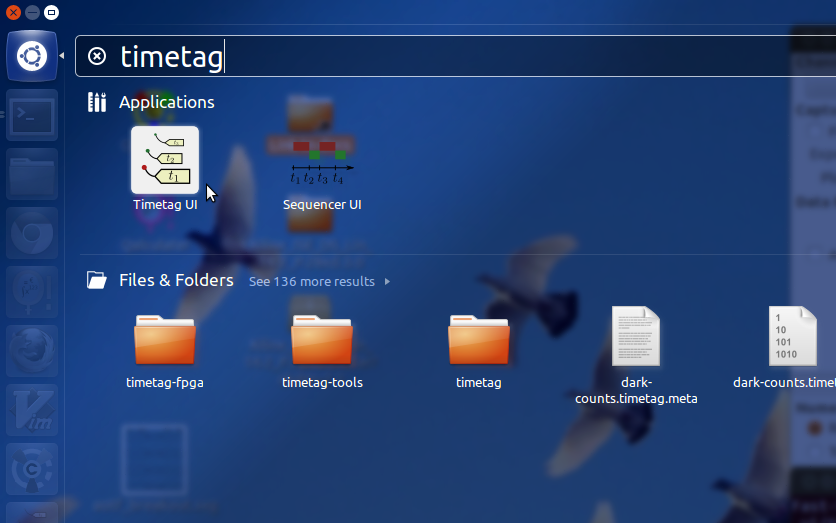
\includegraphics[scale=0.5]{timetag-dash.png}
  \caption{{\tt timetag\_ui} shown in the Ubuntu Dash.}
  \label{Fig:Dash}
\end{figure}

If all of this went smoothly, proceed to the next Chapter where we
will describe basic usage of the software.

\section{Installing {\tt photon-tools}}
\label{Sec:InstallingPhotonTools}

While not strictly necessary for operation of the timetagger, the {\tt
photon-tools} package provides a number of useful utilities for the
analysis of photon timestamp data. This includes basic visualization,
correlation analysis, and modelling software.

Installation is quite straightforward,

\begin{verbatim}
$ sudo apt-get install python python-numpy python-scipy python-matplotlib \
  build-essential cython libboost-all-dev
$ git clone git://github.com/bgamari/photon-tools.git
$ cd photon-tools
$ ./install.sh
\end{verbatim}

Usage of the individual tools is described in the {\tt readme.mkd}
file provided in the {\tt photon-tools} directory.
